\subsubsection{Pending Review Report Management}
\label{sec:pending-review-report-management}

Unlike the previously described functional areas, this area is accessible only to administrative users, who are responsible for supervising ordinary employees. Within this area, administrators can view all pending reports and their associated expenses, and decide whether to approve or reject them. All use cases are represented in the diagram shown in Figure \ref{fig:pending-review-report-management-use-case-diagram}.

\begin{figure}[H]
    \centering
    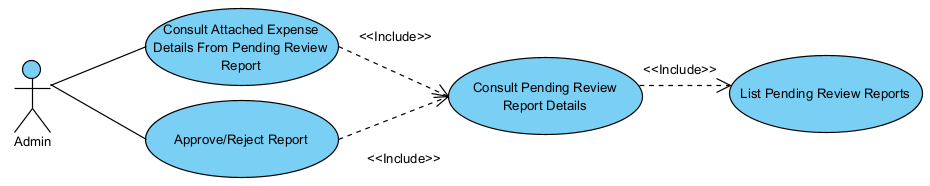
\includegraphics[width=\textwidth]{Images/pendingreviewreportmanagement.png}
    \caption[Pending review report management use case diagram]
    {Pending review report management use case diagram. [Own creation]}
    \label{fig:pending-review-report-management-use-case-diagram}
\end{figure}

\textbf{Use Case: Approve/Reject Report}

\textbf{Primary Actor:} Administrator

\textbf{Trigger:} The administrator approves or rejects a report pending review.

\textbf{Preconditions:} The administrator is authenticated, and the system displays the report metadata along with a list of associated expenses.

\textbf{Postconditions:} The system updates the report status according to the administrator's decision.

\vspace{0.5cm}

\textbf{Main Success Scenario:}

\begin{enumerate}[leftmargin=0.75cm, noitemsep]
    \item The administrator approves or rejects the currently displayed report.
    \item The system updates the report status accordingly and notifies the report owner of the review.
\end{enumerate}

\vspace{0.3cm}

\textbf{Extensions:}

\begin{itemize}[label={}, leftmargin=0.75cm, noitemsep]
    \item \textbf{2a. Report Review Error:}
    \begin{itemize}[label={}, leftmargin=0.75cm, noitemsep]
        \item 2a1. An error occurs during the report review due to a database connection error or an internal error.
        \item 2a2. The system notifies the administrator of the error and keeps them on the current report details view.
    \end{itemize}
\end{itemize}